\section{Casi d'uso}

\subsection{Obiettivi}
La sezione 3 Casi d'uso ha come obiettivo l'identificazione e la descrizione di tutti i casi d'uso, ovvero interazioni tra sistema ed attori, individuati dagli analisti nel tempo tramite lo studio del capitolato d'appalto, del dominio, e tramite incontri con il committente.

\subsection{Attori}
Dato che il requisito obbligatorio richiede la costruzione di una pagina di login(probabilmente username e password saranno preimpostati) che presenti un sistema in grado di distinguere un utente umano da un robot, il prodotto presenterà una sola tipologia di utente:\\
\begin{center}
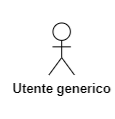
\includegraphics[scale = 1]{img/utente_generico.png}\\
\end{center}
L'utente generico, che potrà essere una persona fisica o anche un bot, potrà accedere a tutte le funzionalità del prodotto. \\
TODO aggiungere eventualmente come utenti il db di unsplash e servizi vari in futuro

\begin{figure}[H]
    \centering
    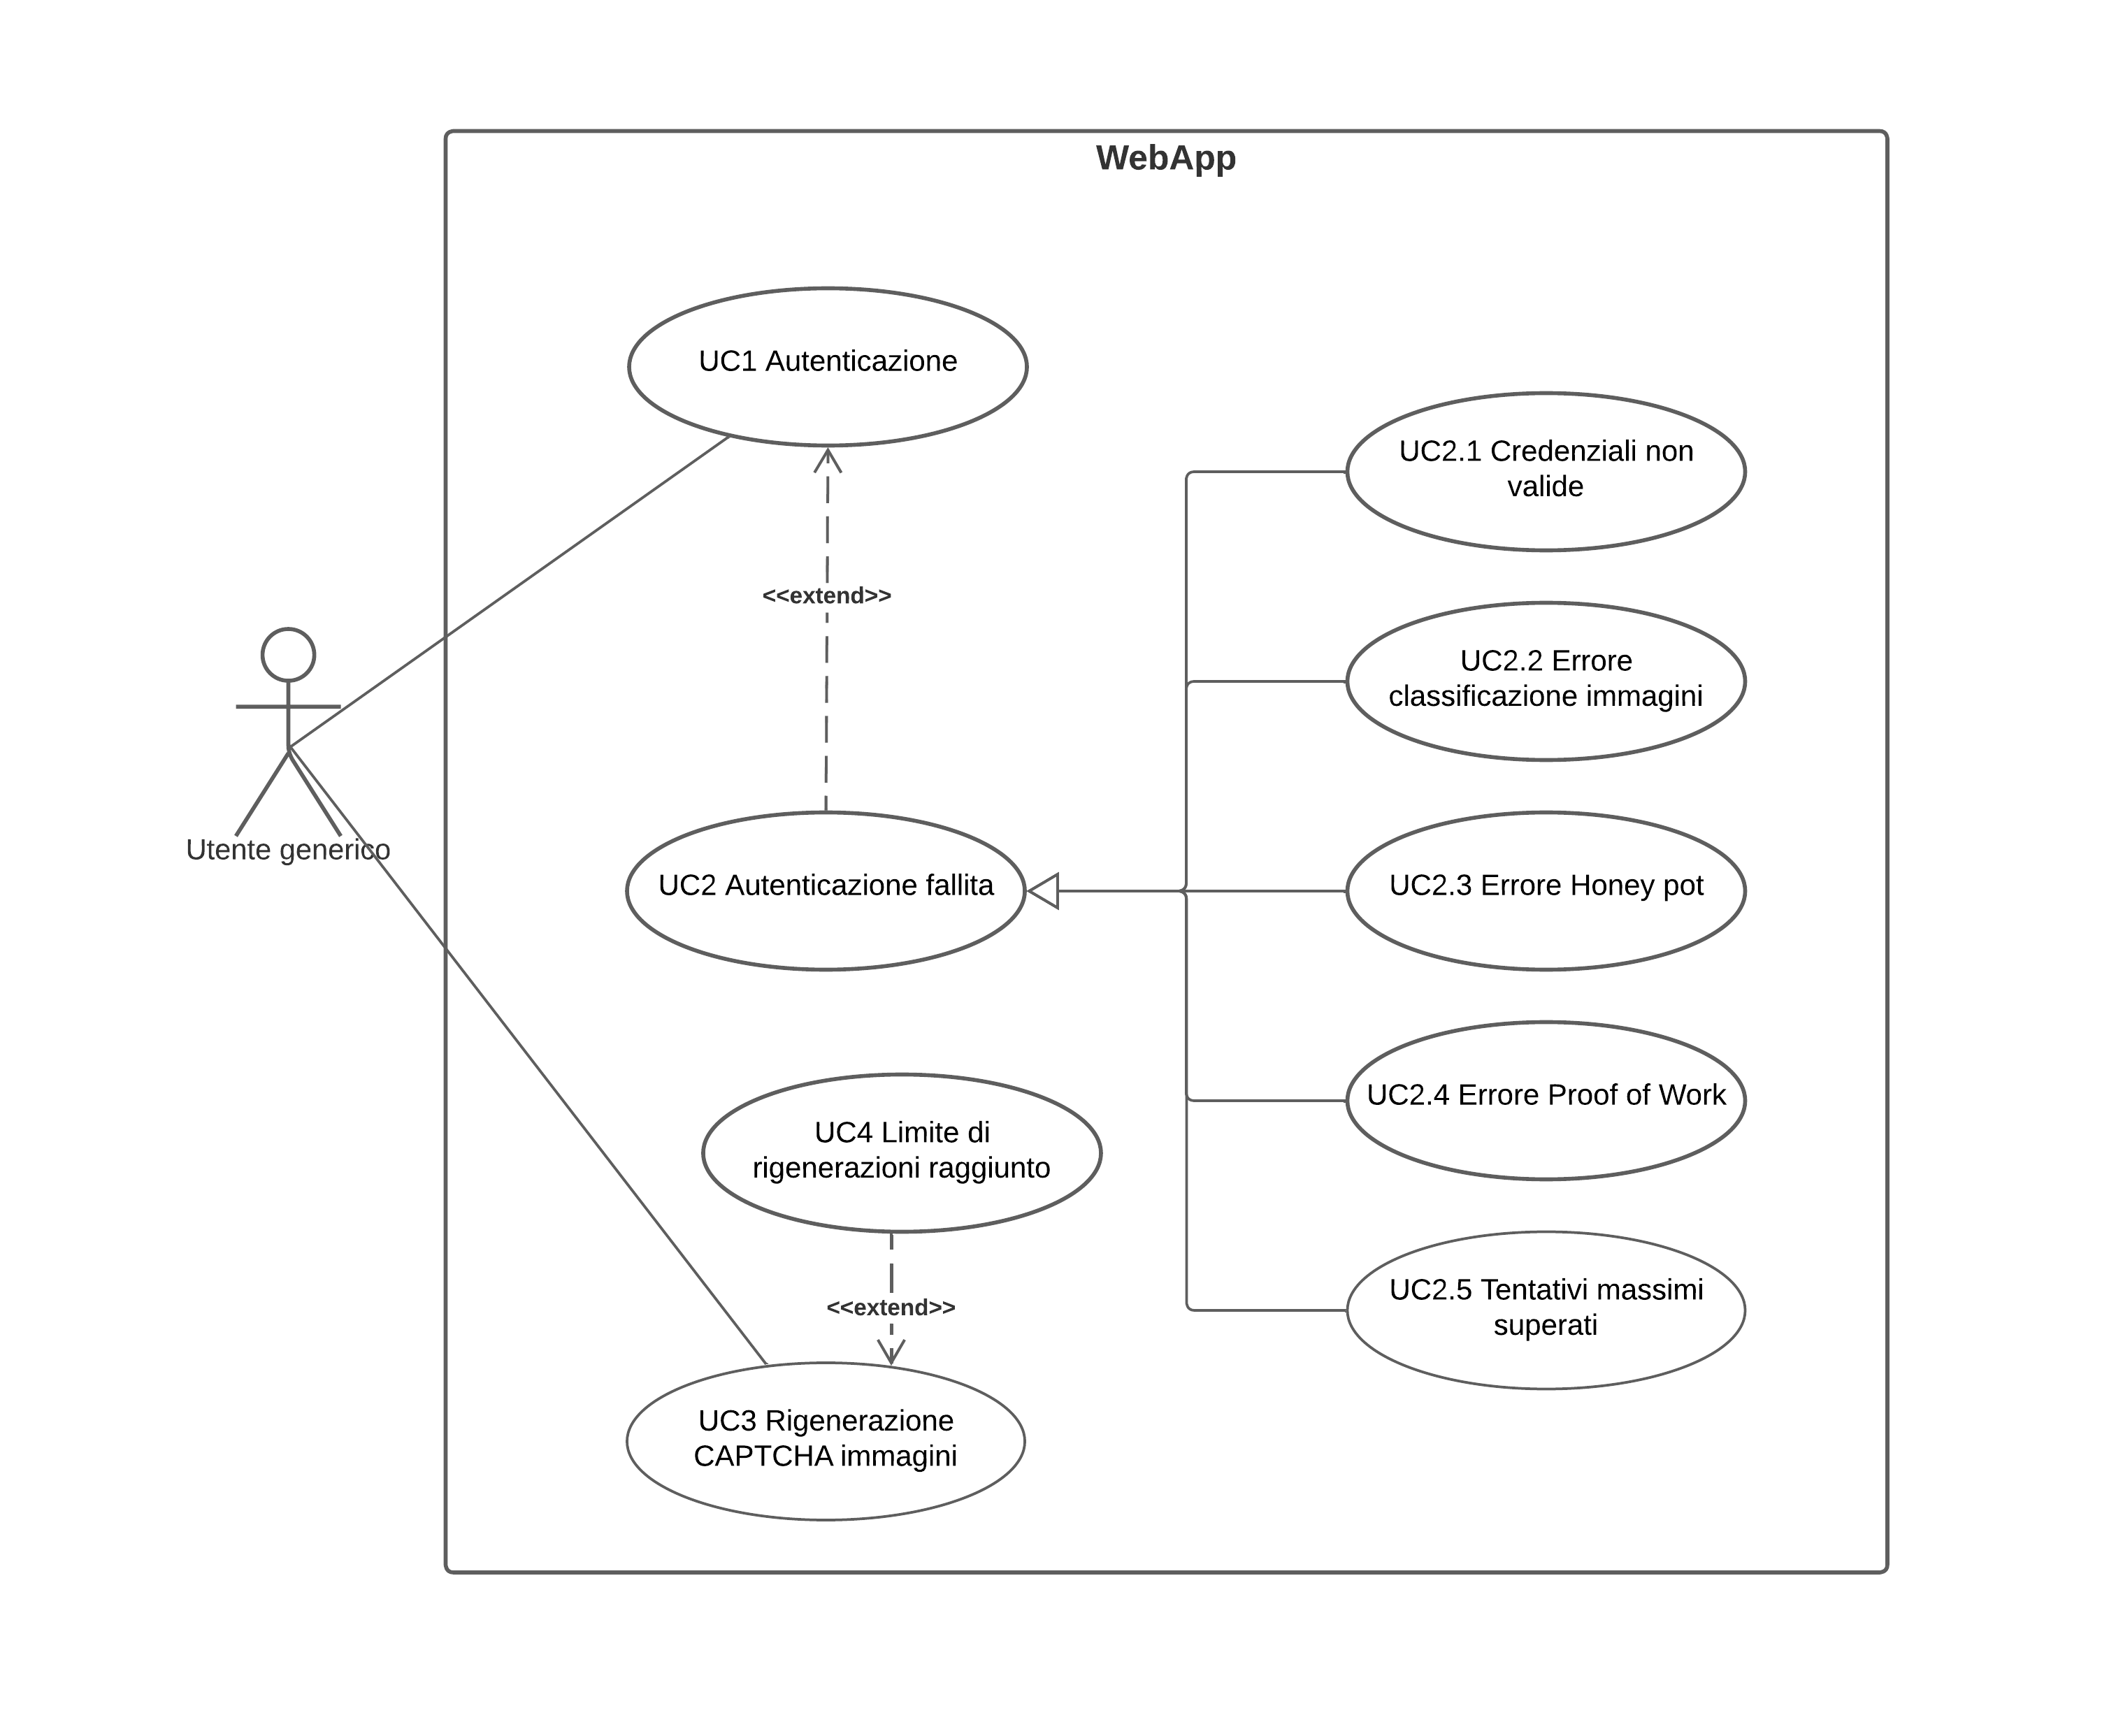
\includegraphics[scale=0.4]{img/web_app.png}
    \caption{Webapp}
\end{figure}
\begin{figure}[H]
    \centering
    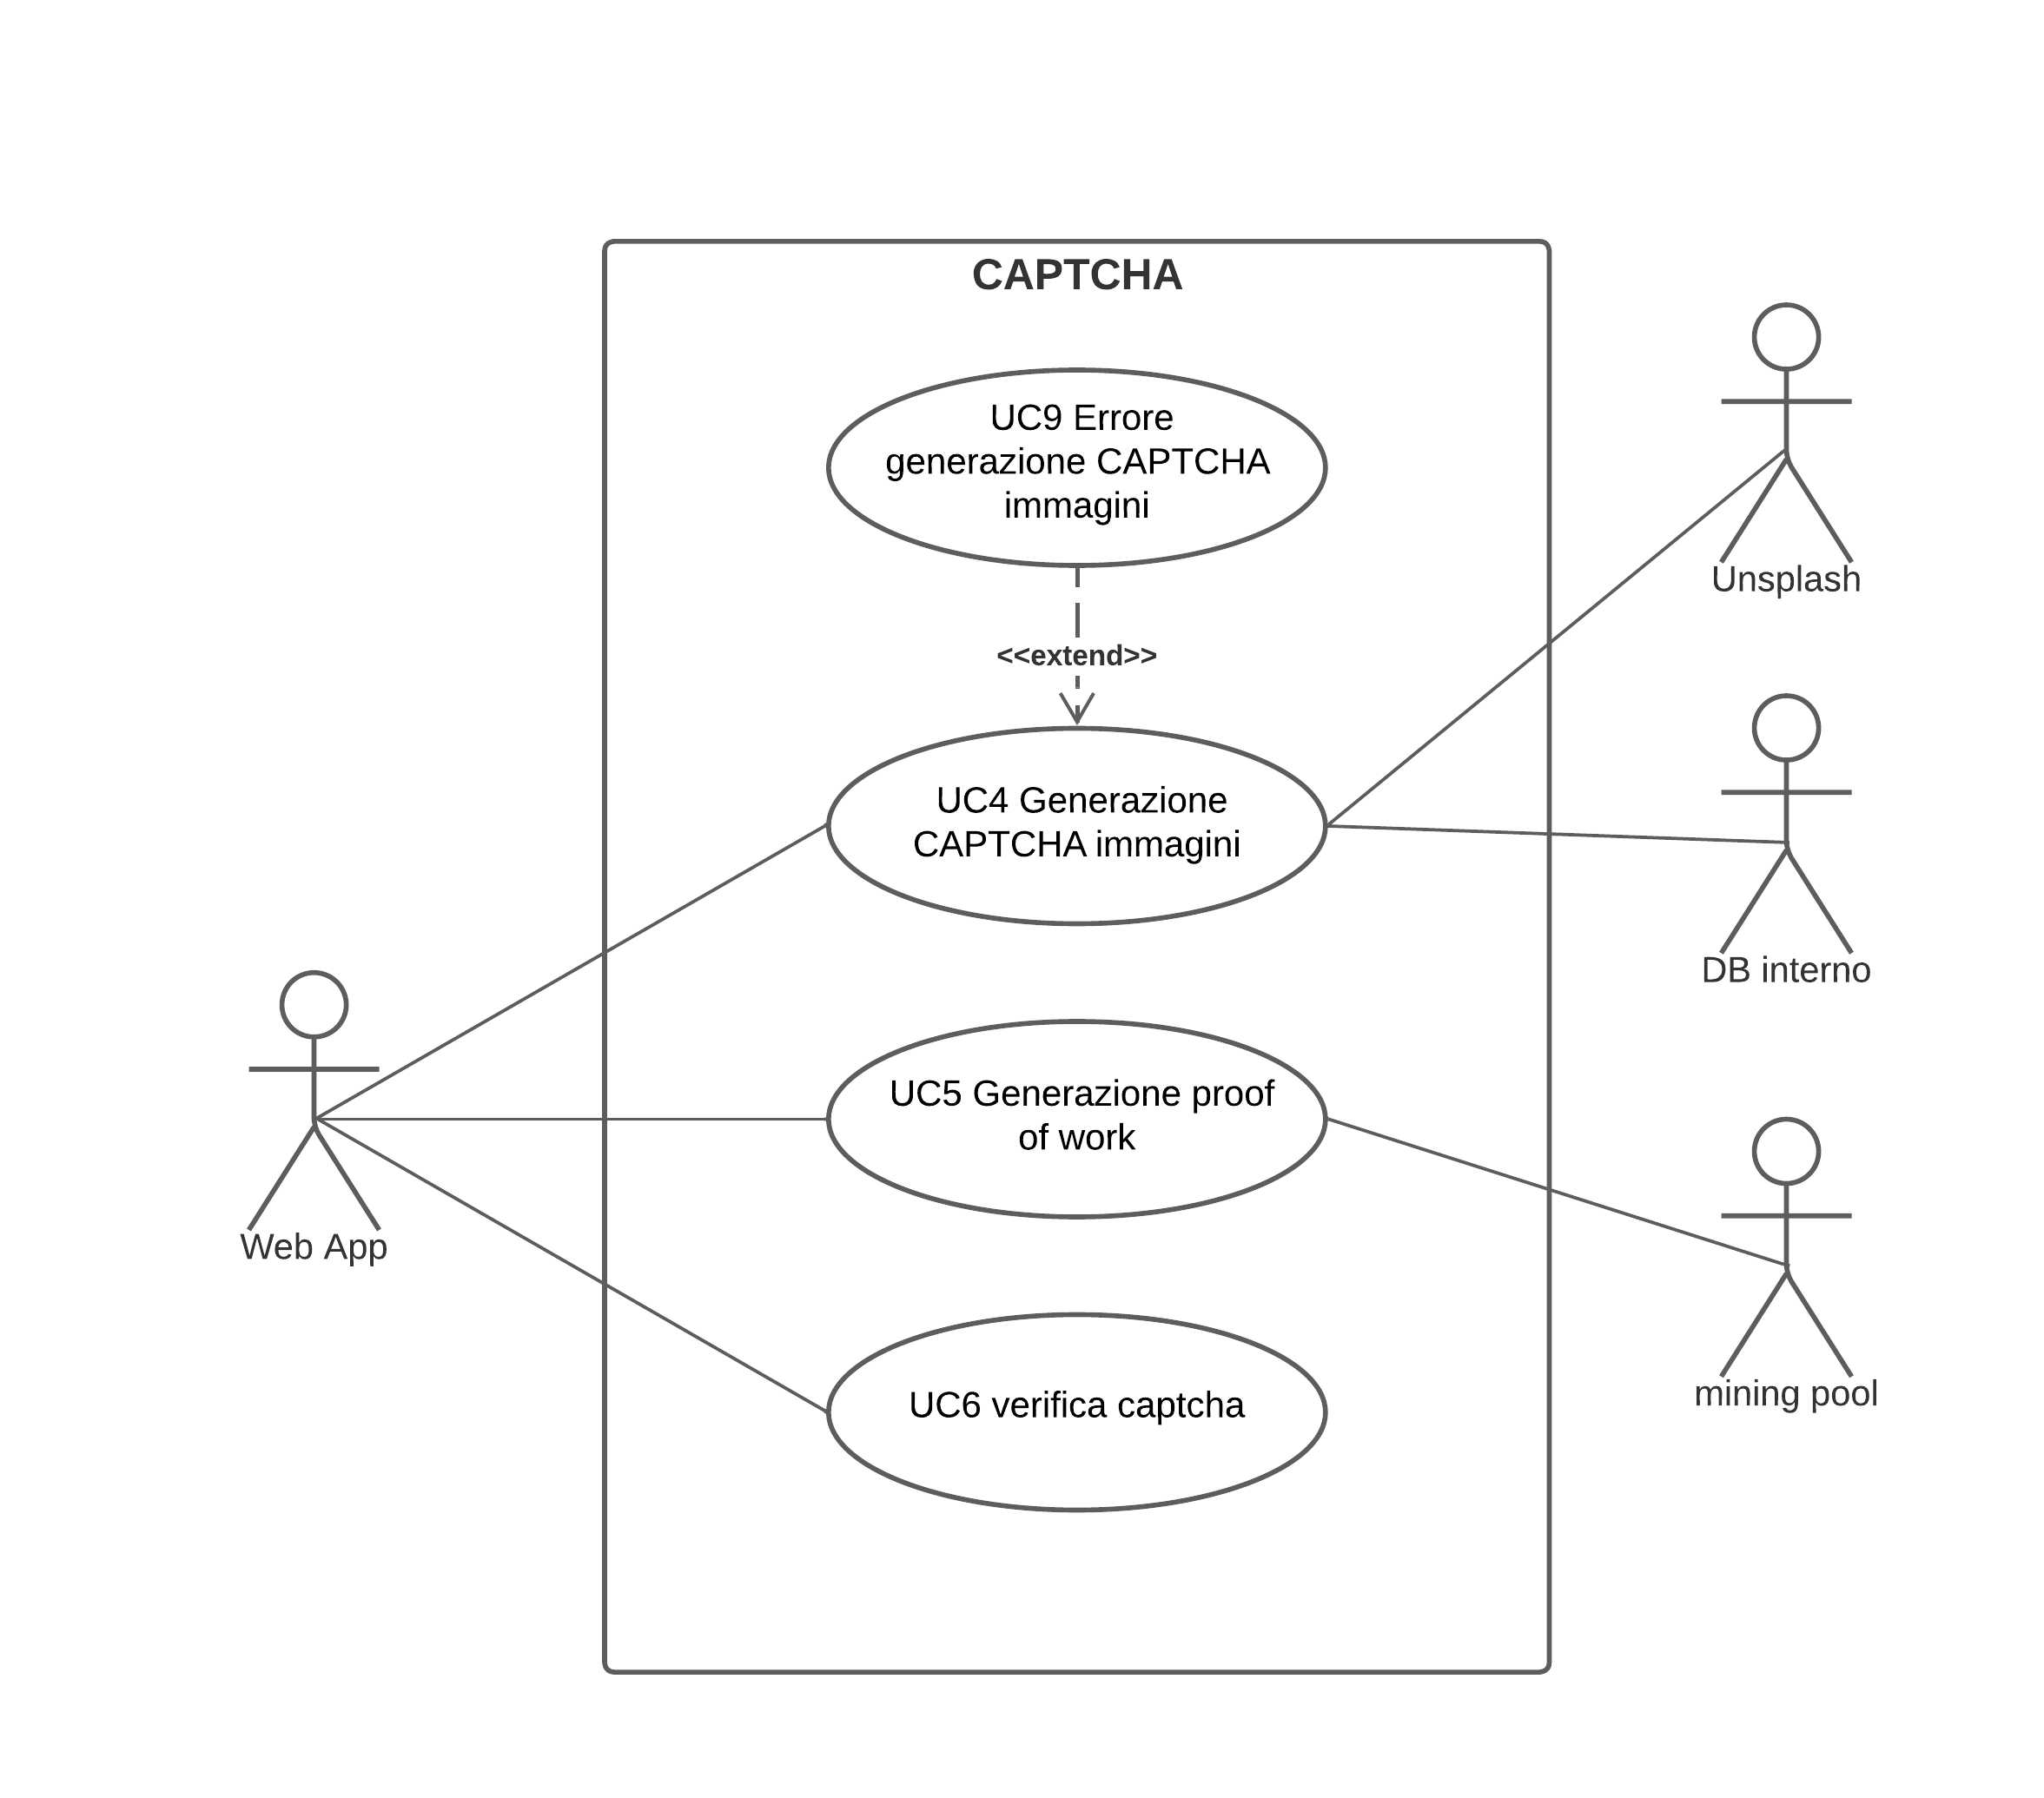
\includegraphics[scale=0.4]{img/catpcha.png}
    \caption{Catpcha}
\end{figure}

\subsection{UC1 - Autenticazione}
\textbf{Attore primario}: Utente generico\\
\textbf{Precondizioni}: Il sistema non riconosce l'utente\\
\textbf{Postcondizioni}: L'utente è autenticato nel sistema\\

\textbf{Scenario principale}: L'utente:
\begin{enumerate}
\item Inserisce i credenziali d'accesso [UC1.1]
\item Compilazione catpcha [UC1.2]
\item Superamento honeypot [UC1.3]
\item Calcolato proof of work [UC1.3]
\end{enumerate}

\textbf{Scenari alternativi}:
\begin{enumerate}
    \item L’utente non supera l'autenticazione. [UC2]
\end{enumerate}

\begin{figure}[H]
    \centering
    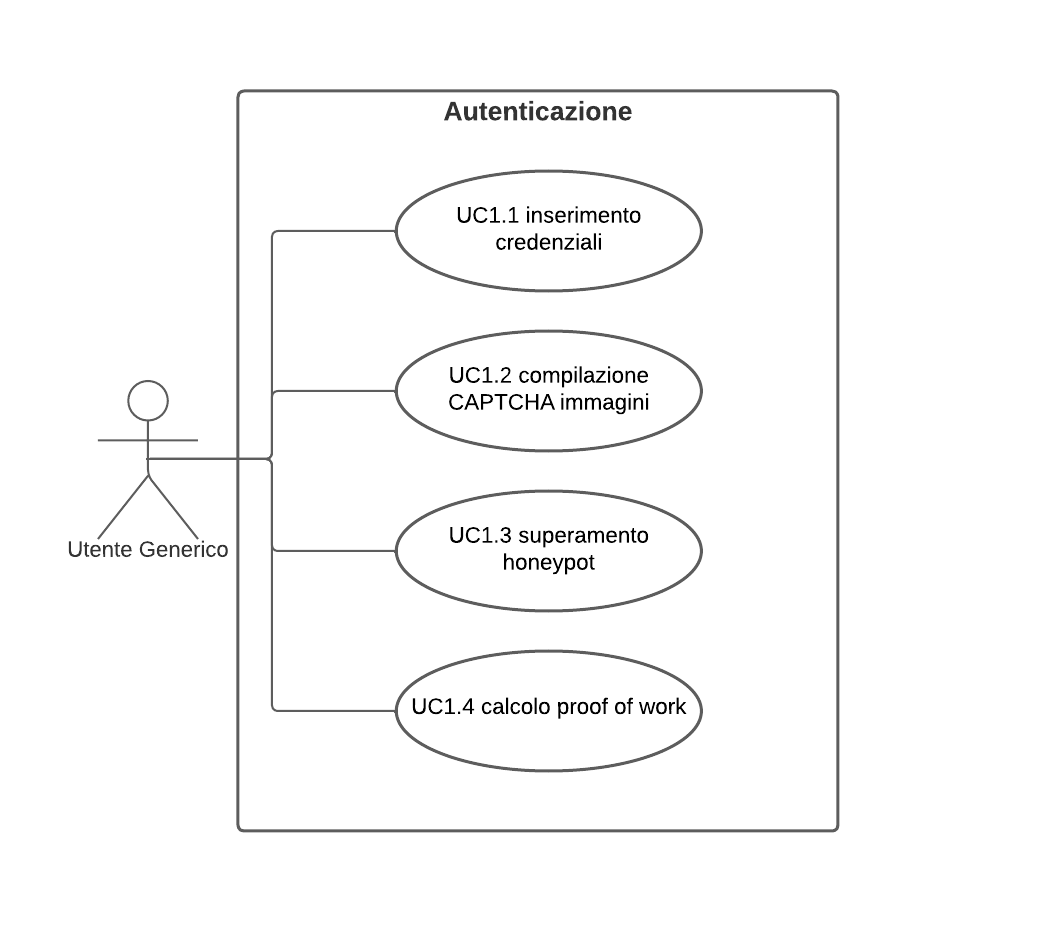
\includegraphics[scale=0.8]{img/Autenticazione.png}
    \caption{UC1-Autenticazione}
\end{figure}

\subsubsection{UC1.1 - Inserimento credenziali d'accesso}
\textbf{Attore primario}: Utente generico\\
\textbf{Precondizioni}: Il sistema non riconosce l'utente e non conosce l'username\\
\textbf{Postcondizioni}: Il sistema ha ricevuto le credenziali dell'utente\\

\textbf{Scenario principale}:
\begin{enumerate}
   \item L'utente inserisce le credenziali negli appositi spazi. Le credenziali devono essere quelli preimpostati.
\end{enumerate}

\subsubsection{UC1.2 - Compilazione captcha}
\textbf{Attore primario}: Utente generico\\
\textbf{Precondizioni}: L'utente visualizza il captcha proposto dal sistema\\
\textbf{Postcondizioni}: L'utente ha risolto il captcha (non necessariamente in modo corretto)\\

\textbf{Scenario principale}:
\begin{enumerate}
   \item L'utente risolve il captcha proposto, non necessariamente in maniera corretta
\end{enumerate}
\textbf{Generalizzazioni}:
\begin{itemize}
   \item captcha tipo 1 [UC1.2.1]
   \item captcha tipo 2 [UC1.2.2]
   \item ...
\end{itemize}

\subsubsection{UC1.3 - Superamento honeypot}
\textbf{Attore primario}: Utente generico\\
\textbf{Precondizioni}: L'utente visualizza il captcha proposto dal sistema\\
\textbf{Postcondizioni}: L'utente ha risolto il captcha (non necessariamente in modo corretto) e non cade nell'honeypot\\

\textbf{Scenario principale}:
\begin{enumerate}
   \item L'utente risolve il captcha proposto, non necessariamente in maniera corretta. Durante la risoluzione non cade nella trappola honeypot.
\end{enumerate}

\subsubsection{UC1.4 - Calcolato il proof of work}
\textbf{Attore primario}: Utente generico\\
\textbf{Precondizioni}: L'utente visualizza il captcha proposto dal sistema\\
\textbf{Postcondizioni}: L'utente ha risolto il captcha (non necessariamente in modo corretto) e viene calcolato il proof of work\\

\textbf{Scenario principale}:
\begin{enumerate}
   \item L'utente risolve il captcha proposto, non necessariamente in maniera corretta. Durante la risoluzione viene calcolato il proof of work.
\end{enumerate}

\paragraph{UC1.3.1 - Compilazione captcha tipo 1 }~\smallskip
\textbf{chiedere quanto si può andare in dettaglio}\\
\textbf{Attore primario}: Utente generico\\
\textbf{Precondizioni}: L'utente visualizza il captcha tipo 1\\
\textbf{Postcondizioni}: L'utente ha completato il captcha di tipo 1\\
\textbf{Scenario principale}:

All'utente viene presentato il captcha tipo 1, con 9 immagini da classificare\\
L'utente classifica le 9 immagini nelle giuste categorie


\paragraph{UC1.3.2 - Compilazione captcha tipo 2}~\smallskip
\textbf{Attore primario}: Utente generico\\
\textbf{Precondizioni}: L'utente visualizza il captcha tipo 2\\
\textbf{Postcondizioni}: L'utente ha completato il captcha di tipo 2\\
\textbf{Scenario principale}:

All'utente viene presentato il captcha tipo 2
[elenco delle azioni che servono per superare il captcha]

\subsection{UC2 - Autenticazione fallita}
\textbf{Attore primario}: Utente generico\\
\textbf{Precondizioni}: L’utente non ha commesso errori di autenticazione.\\
\textbf{Postcondizioni}:L’utente visualizza un messaggio di errore e l’operazione di autenticazione fallisce.\\

\textbf{Scenario principale}:
\begin{enumerate}
   \item L’utente commette un errore nella compilazione del modulo di login.
\end{enumerate}

\textbf{Generalizzazioni}: L'utente ha commesso uno dei seguenti errori:
\begin{enumerate}
	\item Ha inserito delle credenziali errate [UC2.1]
	\item Ha sbagliato la classificazione delle immagini [UC2.2]
	\item Cade nella trappola honeypot [UC2.3]
	\item Non viene calcolato il proof of work [UC2.4]
	\item Ha superato il numero massimo di tentativi disponibili [UC2.5]
\end{enumerate}

\begin{figure}[H]
    \centering
    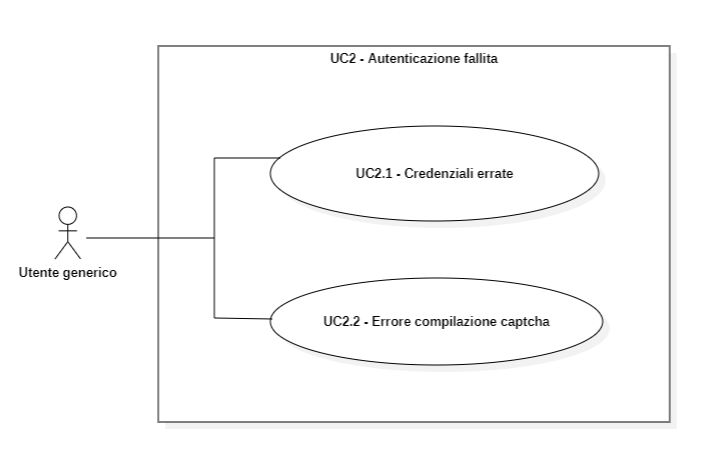
\includegraphics[scale=0.4]{img/Autenticazione_fallita.png}
    \caption{UC2-Autenticazione fallita}
\end{figure}

\subsubsection{UC2.1 - Credenziali errate}
\textbf{Attore primario:} Utente generico\\
\textbf{Precondizioni}: L’utente non ha inserito le credenziali corrette\\
\textbf{Postcondizioni}:  L’utente visualizza un messaggio di errore e l’operazione di autenticazione fallisce. L’utente potrà riprovare  ad autenticarsi.\\

\textbf{Scenario principale}:
\begin{enumerate}
	\item L’utente visualizza un messaggio di errore
	\item L’operazione di autenticazione fallisce
	\item Viene generato un altro captcha e l’utente potrà riprovare ad autenticarsi
\end{enumerate}

\subsubsection{UC2.2 - Errore compilazione captcha}
\textbf{Attore primario:} Utente generico\\
\textbf{Precondizioni}: L’utente non ha compilato correttamente il captcha\\
\textbf{Postcondizioni}:  L’utente visualizza un messaggio di errore e l’operazione di autenticazione fallisce. L’utente potrà riprovare  ad autenticarsi.\\

\textbf{Scenario principale}:
\begin{enumerate}
	\item Viene visualizzato un errore esplicativo
	\item Il numero di tentativi compiuti dall’utente negli ultimi 20 minuti aumenta di 1
	\item L’utente non viene autenticato nel sistema e potrà  riprovare ad autenticarsi
\end{enumerate}

\textbf{Scenario alternativo}:
\begin{enumerate}
	\item L’utente ha superato il numero di tentativi consentito per la compilazione del captcha negli ultimi 20 minuti. [UC3]
\end{enumerate}

\subsubsection{UC2.3 - Trappola honeypot selezionata}
\textbf{Attore primario:} Utente generico\\
\textbf{Precondizioni}: L’utente ha selezionato l'immagine nascosta\\
\textbf{Postcondizioni}:  L’utente visualizza un messaggio di errore e l’operazione di autenticazione fallisce. L’utente verrà riconosciuto come bot e non potrà riprovare  ad autenticarsi.\\

\textbf{Scenario principale}:
\begin{enumerate}
	\item L’utente visualizza un messaggio di errore
	\item L’operazione di autenticazione fallisce
	\item Viene riconosciuto come bot e verrà bloccato per futuri tentativi
\end{enumerate}

\subsubsection{UC2.4 - Non viene calcolato il proof of work}
\textbf{Attore primario:} Utente generico\\
\textbf{Precondizioni}: La compilazione delle credenziali e del catpcha troppo rapida. Non viene eseguito il calcolo del proof of work\\
\textbf{Postcondizioni}:  L’utente visualizza un messaggio di errore e l’operazione di autenticazione fallisce. L’utente verrà riconosciuto come bot e non potrà riprovare  ad autenticarsi.\\

\textbf{Scenario principale}:
\begin{enumerate}
	\item L’utente visualizza un messaggio di errore
	\item L’operazione di autenticazione fallisce
	\item Viene riconosciuto come bot e verrà bloccato per futuri tentativi
\end{enumerate}

\subsubsection{UC2.5 - Superamento tentativi consentiti}
\textbf{Attore primario:} Utente generico\\
\textbf{Precondizioni}: L'utente supera le autenticazioni precedenti ma finisce i tentativi disponibili\\
\textbf{Postcondizioni}:  L’utente visualizza un messaggio di errore e l’operazione di autenticazione fallisce. L’utente potrà riprovare ad autenticarsi più tardi.\\

\textbf{Scenario principale}:
\begin{enumerate}
	\item L’utente visualizza un messaggio di errore
	\item L’operazione di autenticazione fallisce
	\item L’utente non viene autenticato nel sistema e potrà  riprovare ad autenticarsi più tardi
\end{enumerate}

\subsection{UC3 - Rigenerazione captcha immagini}
\textbf{Attore primario}: Utente generico\\
\textbf{Precondizioni}: L'utente non riconosce le immagini e richiere la generazione di un altro set di immagini\\
\textbf{Postcondizioni}:Viene generato un nuovo set di immagini e l'utente continua con l'autenticazione\\

\textbf{Scenario principale}:
\begin{enumerate}
   \item L'utente non riesce a compilare il captcha
   \item L'utente richiede un altro set di immagini
   \item Viene generato un altro set di immagini
   \item Viene decrementato di uno il numero di tentativi
   \item L'utente continua con la compilazione del captcha
\end{enumerate}

\subsection{UC4 - Generazione di un altro captcha (da chiedere su una possibile generalizzazione)}
\textbf{Attore primario}: Utente generico\\
\textbf{Precondizioni}: L'utente ha visualizzato il captcha proposto\\
\textbf{Postcondizioni}: All'utente viene proposto un nuovo captcha\\

\textbf{Scenario principale}:
\begin{enumerate}
   \item L'utente richiede la generazione di un nuovo captcha
   \item Il sistema propone all'utente un altro captcha
\end{enumerate}

\begin{figure}[H]
    \centering
    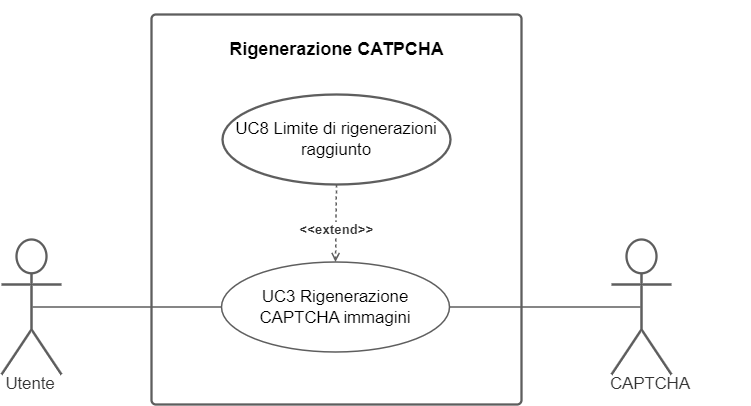
\includegraphics[scale=0.6]{img/Generazione_catpcha.png}
    \caption{UC3-Generazione CATPCHA}
\end{figure}